\documentclass{article}
\usepackage[utf8]{inputenc}

\usepackage[english]{babel}
\usepackage[utf8x]{inputenc}

\usepackage{multicol}
\usepackage[vmargin=3cm,hmargin=4cm]{geometry}
\usepackage{parskip}
\usepackage[runin]{abstract}
\renewcommand{\abstitleskip}{0mm}
\usepackage{hyperref}
\usepackage{lmodern}
\usepackage[T1]{fontenc}
\usepackage{caption}
\usepackage{subcaption}
\usepackage{graphicx}
\usepackage{ccaption}
\captionnamefont{\it}
\captiontitlefont{\it}
\usepackage{enumitem}
\usepackage{qtree}

\usepackage{capt-of}
\usepackage{float}
\usepackage{listings}

\usepackage[toc,page]{appendix}


\usepackage{amsmath}
\usepackage{amsthm}

\makeatletter

\title{Homework 1}
\author{Martin Karp\\Advanced Methods for Numerical Fluid Dynamics\\ MVKN70}
\renewcommand*\maketitle{
  {
    \begin{center}
      {\huge\bfseries \@title}\\
      \vspace{5mm}
      {\large \@author}
    \end{center}
    \vspace{2mm}
  }
}
\makeatother

\begin{document}
\maketitle

\section*{Task 1}
For each method and equation a plot is provided with the initial state in blue and the state after one time step in orange. The result is provided with 3 decimal points of accuracy.

The methods all give "similar' results, but with somewhat varying amplitude. The largest difference is that some methods depend on the centralized difference while others do not. This manifests itself in that some schemes change the value of no only indices 3 and 7. However, the general trend of a right going wave is maintained in all solutions.

Especially the Godunov scheme and Roe scheme behave exactly in the same way. This was also said to be the case in the lecture for waves going in the same direction, hopefully we will observe a different result when the waves go both to the right and left.

As for the Roe-Fromm scheme it is quite different to all the other schemes because of the central linear extrapolation that is used.  Also a weird thing is that the solution for the Burgers equation exhibit less symmetry than the other schemes.

\subsection*{Monotonicity}
The methods behave quite differently with regard to monotonicity, however as expected all first order methods maintain this property. The second order methods do however, not keep the monotonicity in general. This is in line with the lecture and caused by the numerical under/overshoots that occur in second order methods.

\subsection*{}


\begin{figure}[H]
  \centering
  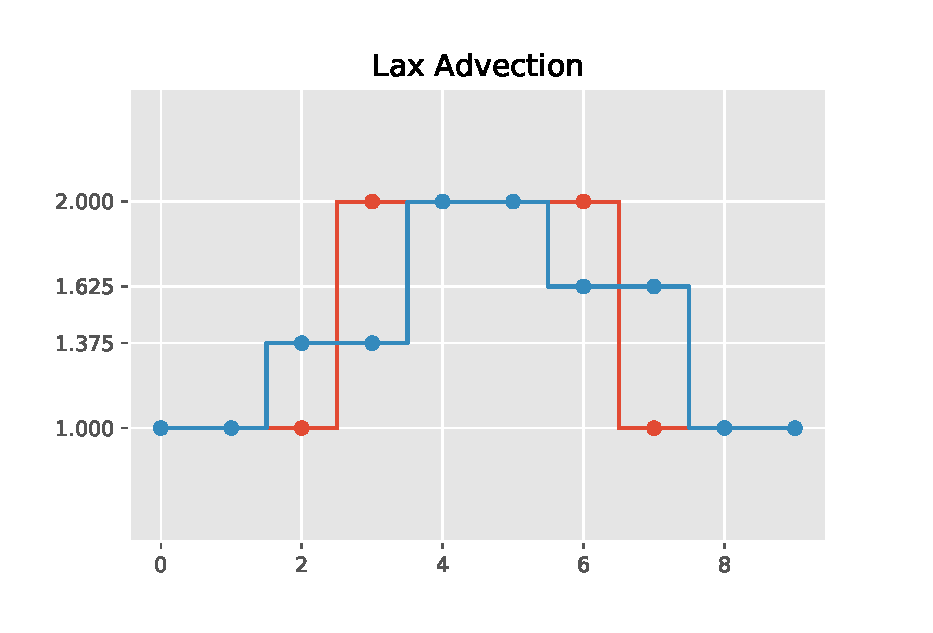
\includegraphics[width=1\linewidth]{pics/LAXadvection.eps}
  \label{fig:perf}
 \end{figure}

\begin{figure}[H]
  \centering
  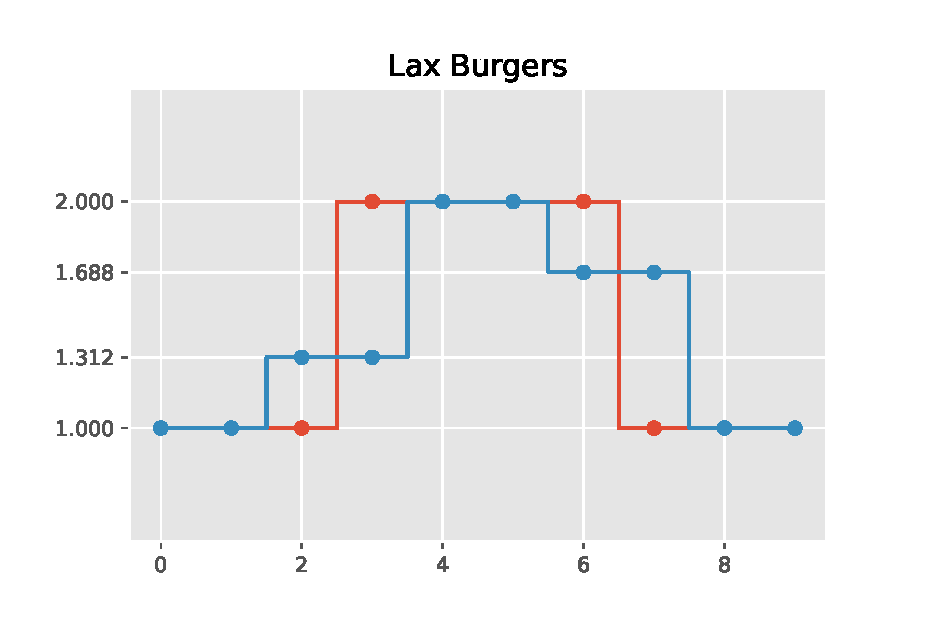
\includegraphics[width=1\linewidth]{pics/LAXburger.eps}
  \label{fig:perf}
 \end{figure}

 \begin{figure}[H]
  \centering
  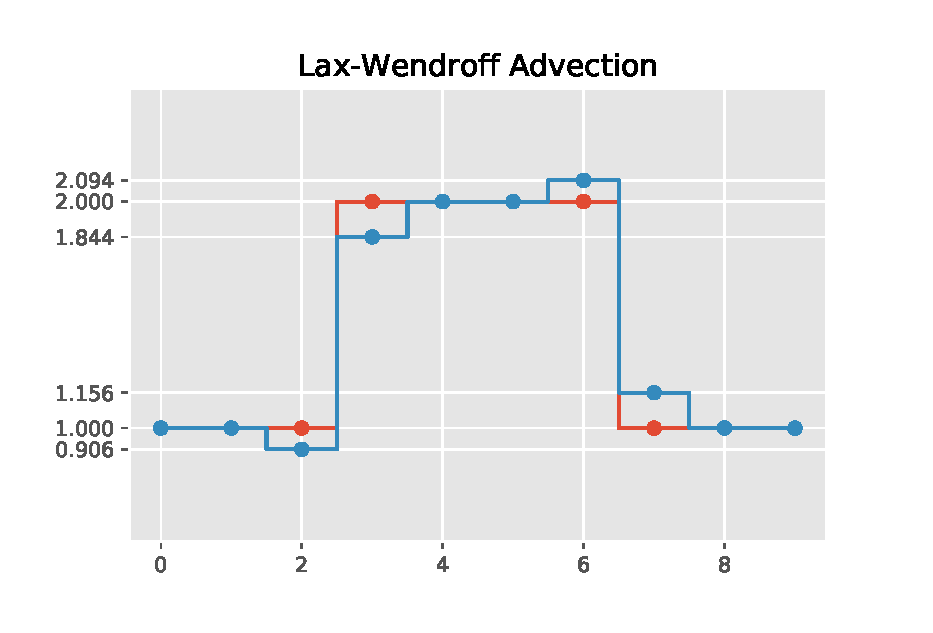
\includegraphics[width=1\linewidth]{pics/Wendroffadvection.eps}
  \label{fig:perf}
  \end{figure}

  \begin{figure}[H]
  \centering
  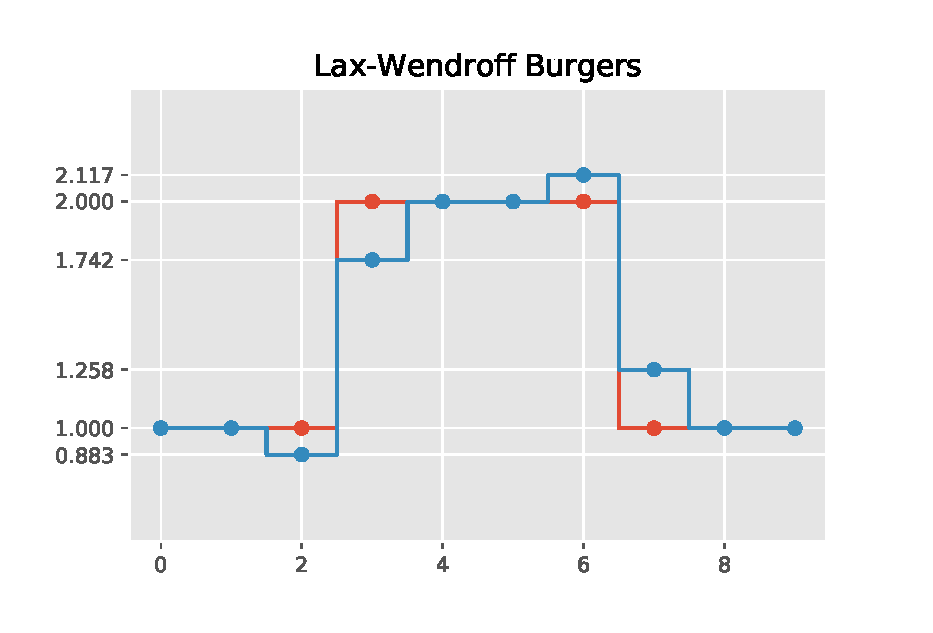
\includegraphics[width=1\linewidth]{pics/Wendroffburger.eps}
  \label{fig:perf}
 \end{figure}

\begin{figure}[H]
  \centering
  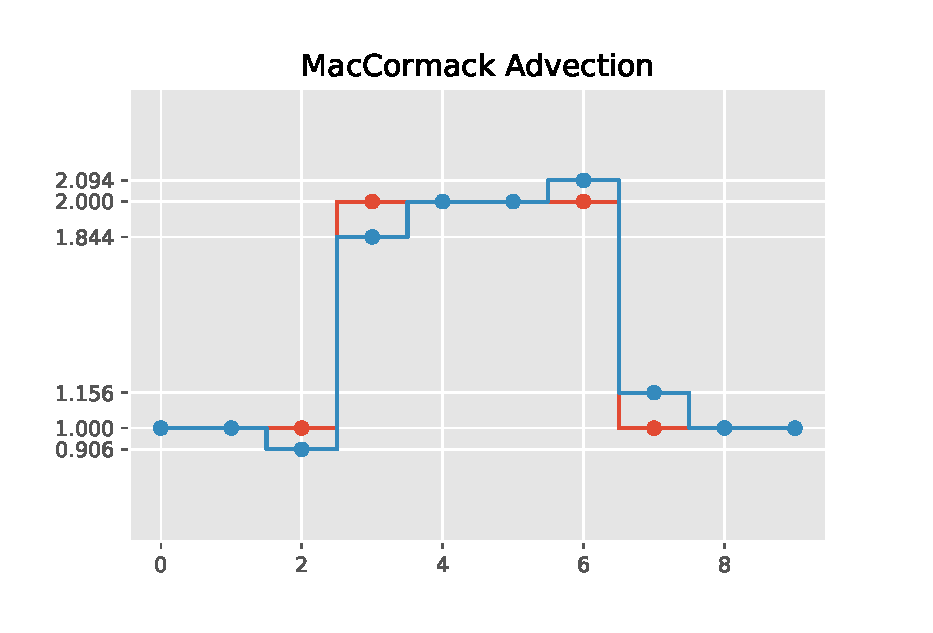
\includegraphics[width=1\linewidth]{pics/Maccormackadvection.eps}
  \label{fig:perf}
 \end{figure}

 \begin{figure}[H]
  \centering
  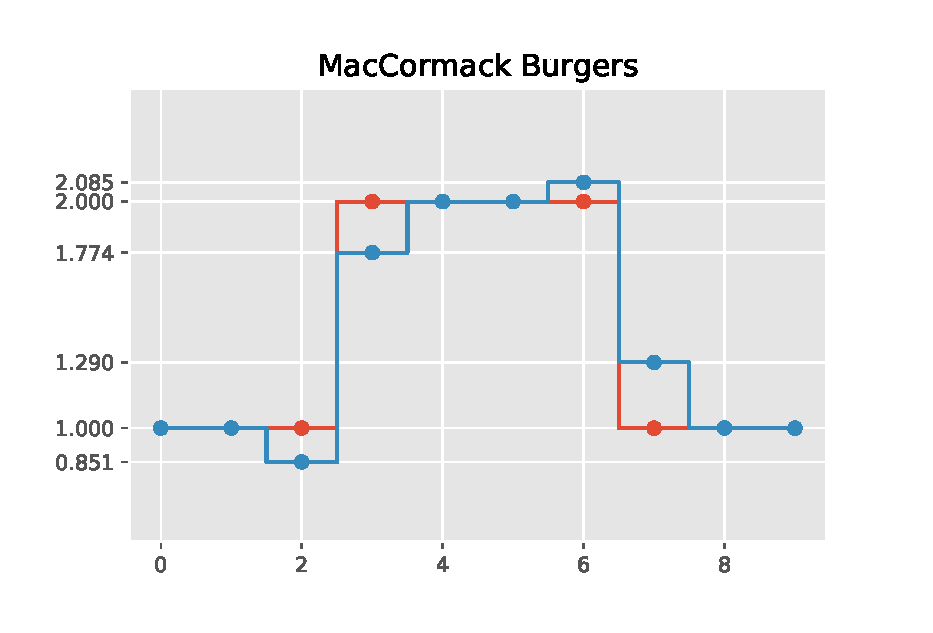
\includegraphics[width=1\linewidth]{pics/Maccormackburgers.eps}
  \label{fig:perf}
 \end{figure}

  \begin{figure}[H]
  \centering
  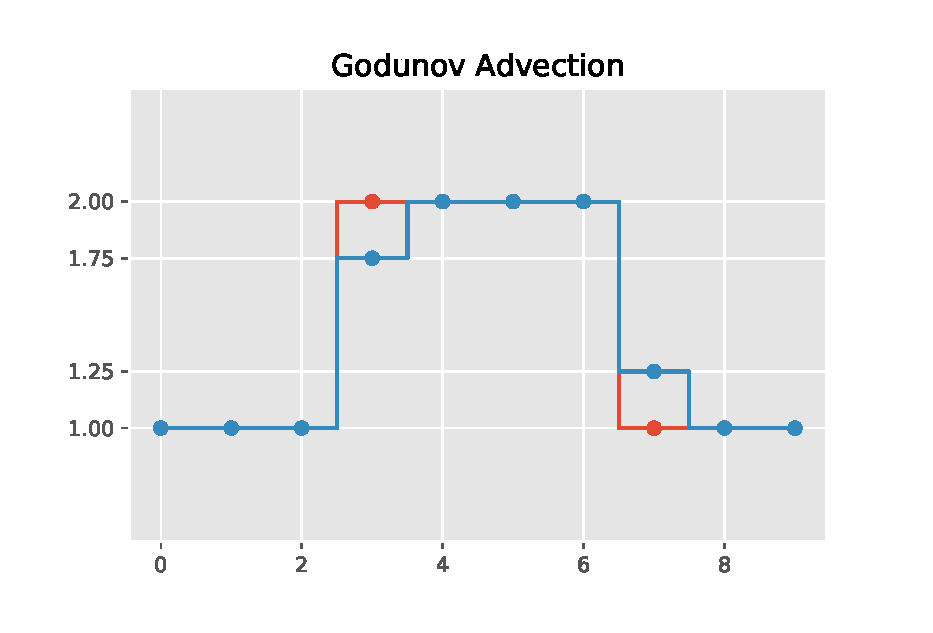
\includegraphics[width=1\linewidth]{pics/Godunovadvection.eps}
  \label{fig:perf}
 \end{figure}

  \begin{figure}[H]
  \centering
  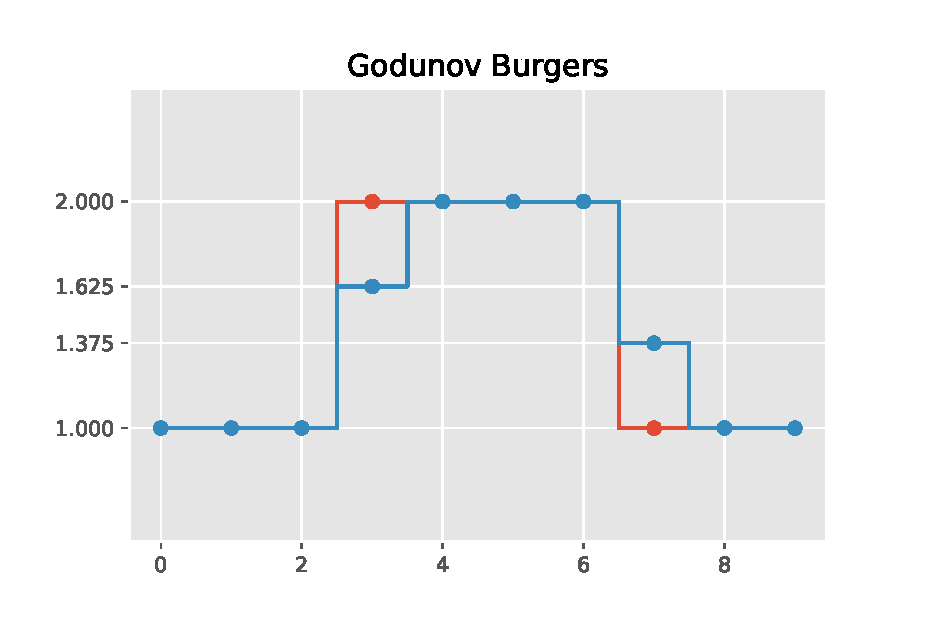
\includegraphics[width=1\linewidth]{pics/Godunovburgers.eps}
  \label{fig:perf}
 \end{figure}

  \begin{figure}[H]
  \centering
  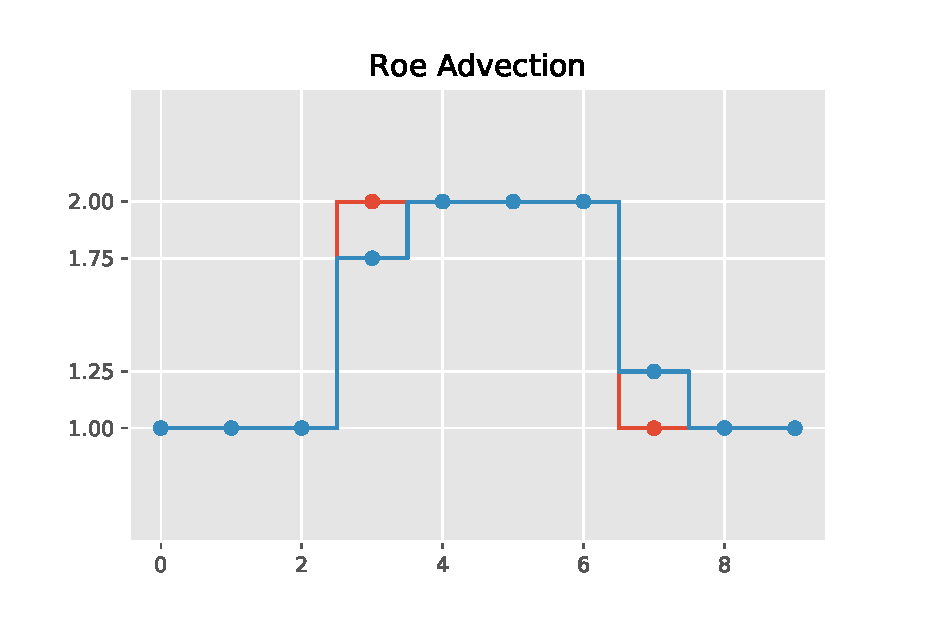
\includegraphics[width=1\linewidth]{pics/Roeadvection.eps}
  \label{fig:perf}
 \end{figure}

  \begin{figure}[H]
  \centering
  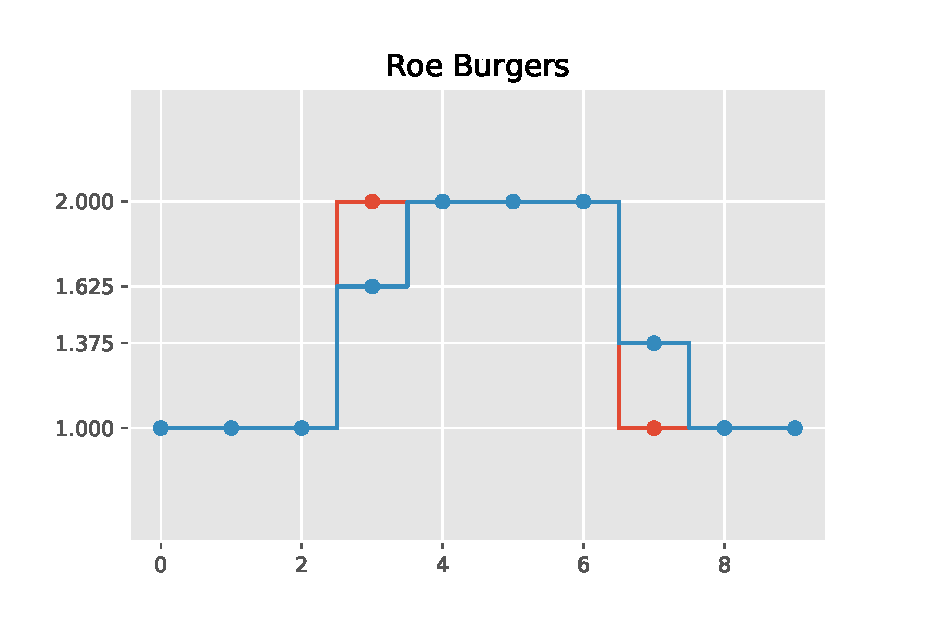
\includegraphics[width=1\linewidth]{pics/Roeburgers.eps}
  \label{fig:perf}
 \end{figure}

 \begin{figure}[H]
  \centering
  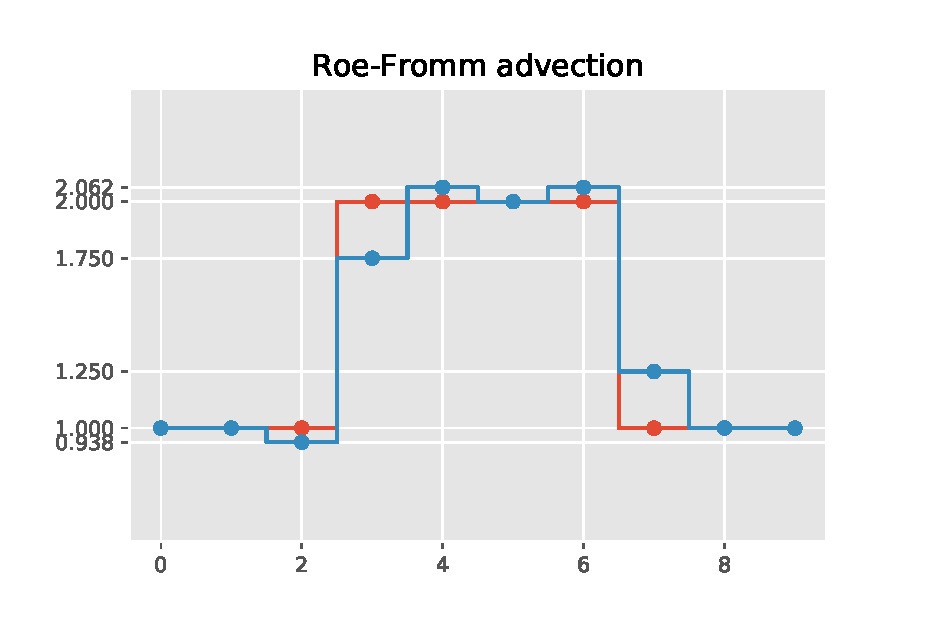
\includegraphics[width=1\linewidth]{pics/Roefrommadvection.eps}
  \label{fig:perf}
 \end{figure}

 \begin{figure}[H]
  \centering
  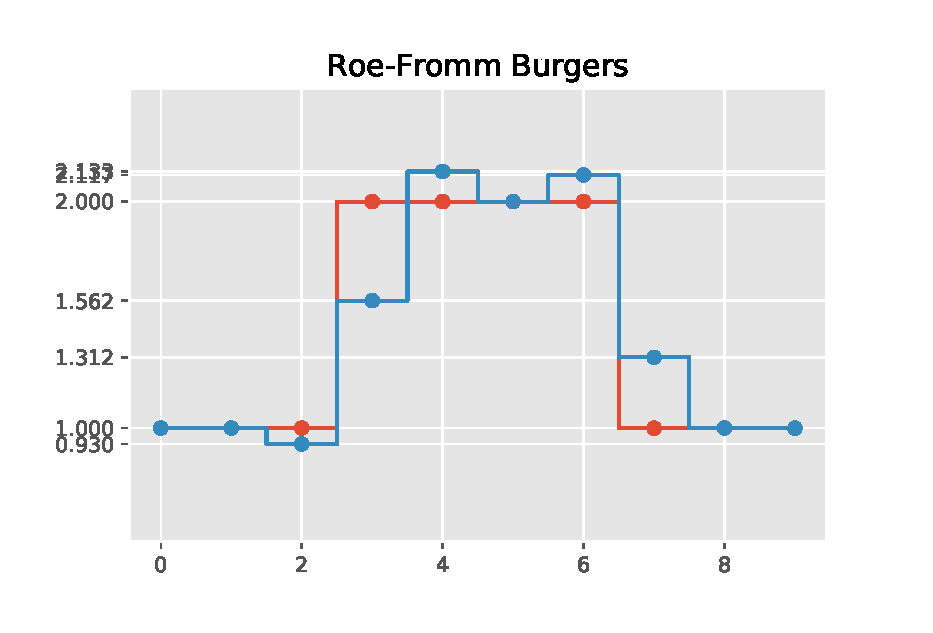
\includegraphics[width=1\linewidth]{pics/Roefrommburgers.eps}
  \label{fig:perf}
 \end{figure}

\section*{Task 2}
Here the results for advection are still exactly the same while the solution for the Burgers equation differ.

As previously mentioned we did expect slightly different results from the Roe and Godunov scheme. This is because the simplification in Roe will lead to a less accurate propagation of the wave and will not properly display the expansion wave that occurs. This leads to index 3 for example having a higher amplitude than in Godunov. This is similar to the example in the lecture.

\begin{figure}[H]
  \centering
  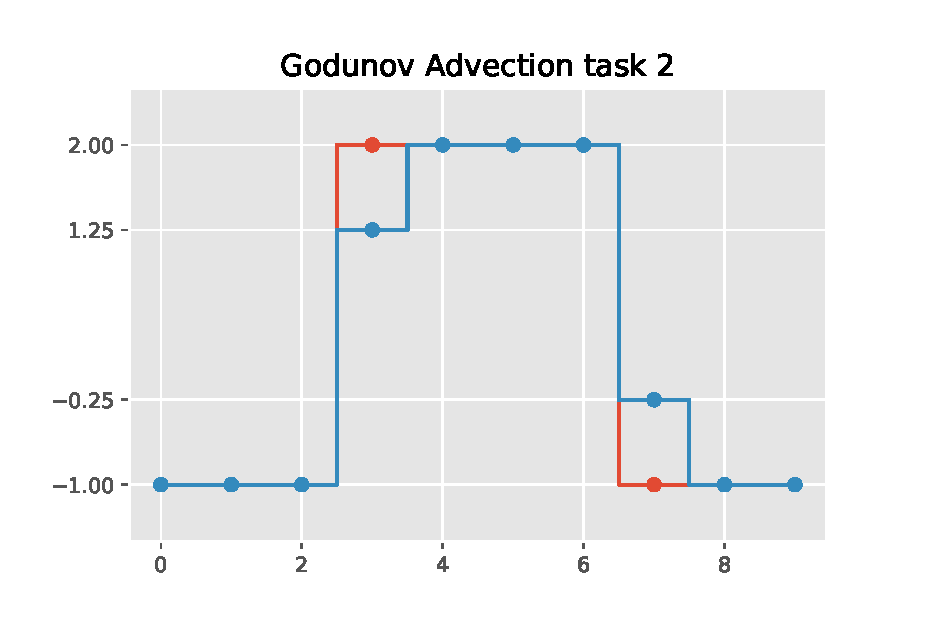
\includegraphics[width=1\linewidth]{pics/Godunovadvection2.eps}
  \label{fig:perf}
 \end{figure}

\begin{figure}[H]
  \centering
  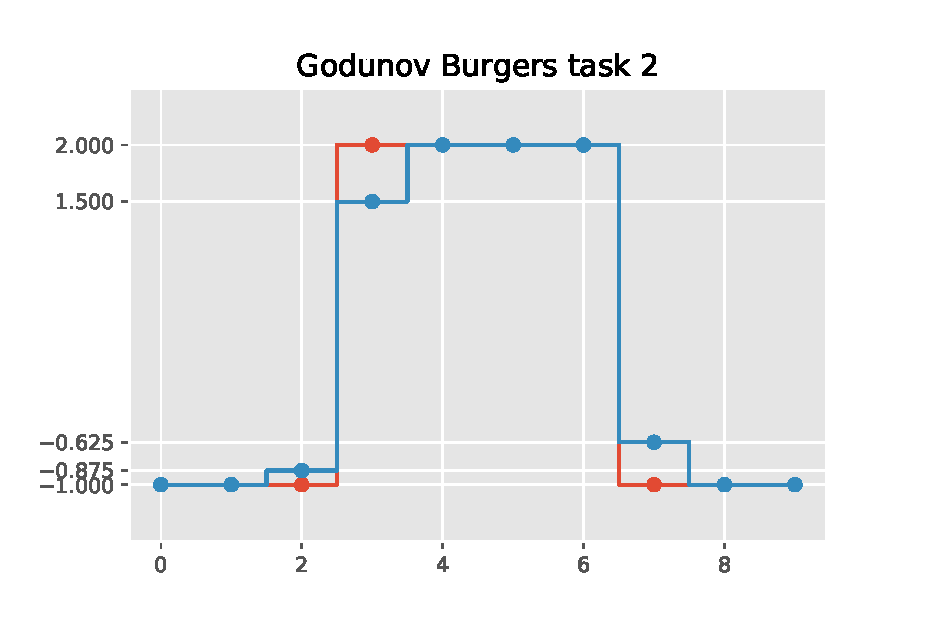
\includegraphics[width=1\linewidth]{pics/Godunovburgers2.eps}
  \label{fig:perf}
 \end{figure}

 \begin{figure}[H]
  \centering
  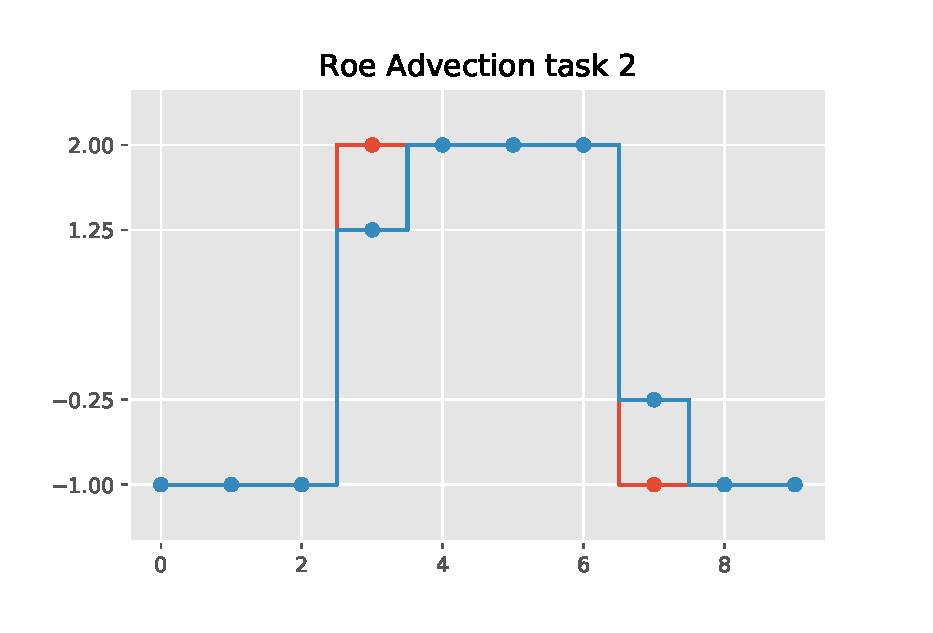
\includegraphics[width=1\linewidth]{pics/Roeadvection2.eps}
  \label{fig:perf}
 \end{figure}

 \begin{figure}[H]
  \centering
  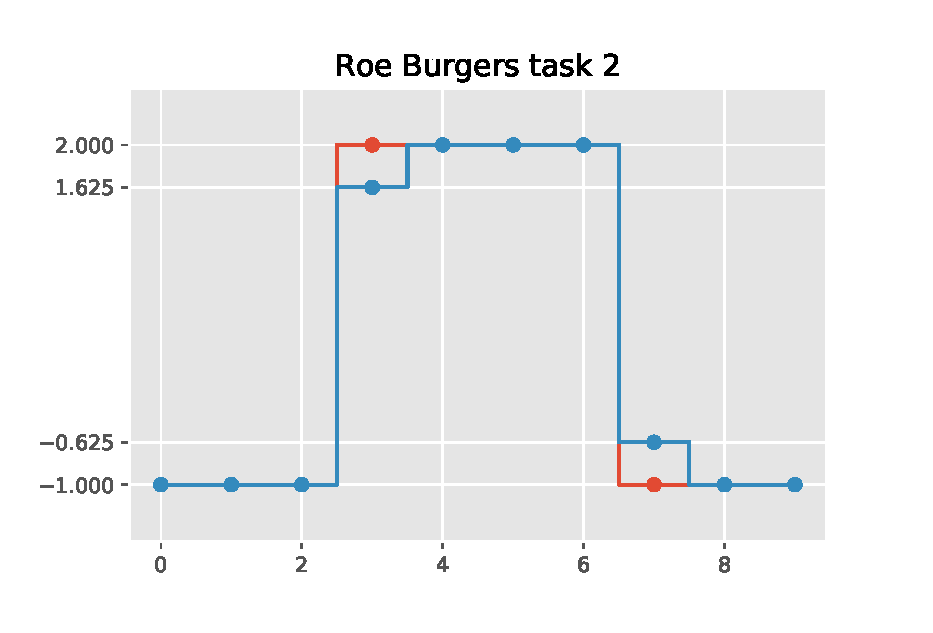
\includegraphics[width=1\linewidth]{pics/Roeburgers2.eps}
  \label{fig:perf}
 \end{figure}

\end{document}
